%$Id: geometry.tex,v 1.1 1992/05/10 19:38:58 rz Exp rz $
\chapter{Computations in Algebraic Geometry}
\label{Geometry:Chap}


Although this book discusses algorithms for manipulating symbolic and
algebraic quantities, there is a great deal to be gained by examining
these calculations from a geometric point of view.  In this chapter we
discuss the geometry which underlies our polynomial computations.  In
doing this we will be significantly more mathematically rigorous than
we were in the previous chapter.  This has a significant advantage in
that it will allow us to apply our geometric intuition in arenas where
the geometry is not clear, in particular in the case of finite fields.
In many ways this chapter and the previous one reflect the
chronological development of algebra.  The previous chapter is the
algebra of {\Cayley}, {\Sylvester} and {\Gordan}, the pre-1890 masters.
This chapter is the algebra of {\Hilbert}, E. {\NoetherE} and
{\Waerden} the creators of what is often called {\em modern
algebra\/}.

We begin with some basic definitions and theorems in commutative algebra
so that we will have a vocabulary to discuss the geometrical objects
that come later.  The bulk of the chapter discusses different techniques
for extracting information from an ideal, which is the central object
discussed.


\section{Geometry}
\label{Geometry:Sec}

In this section we will give some concrete examples of the geometrical
ideas we want to talk about later.  As usual when we speak of a
commutative ring, we will mean a commutative ring with a
multiplicative identity.  In the next few pages we will be playing
pretty fast and loose with some of the definitions while we try to
establish some intuition.  Later we will make these concepts more
precise and accurate.

\begin{figure}
\begin{center}
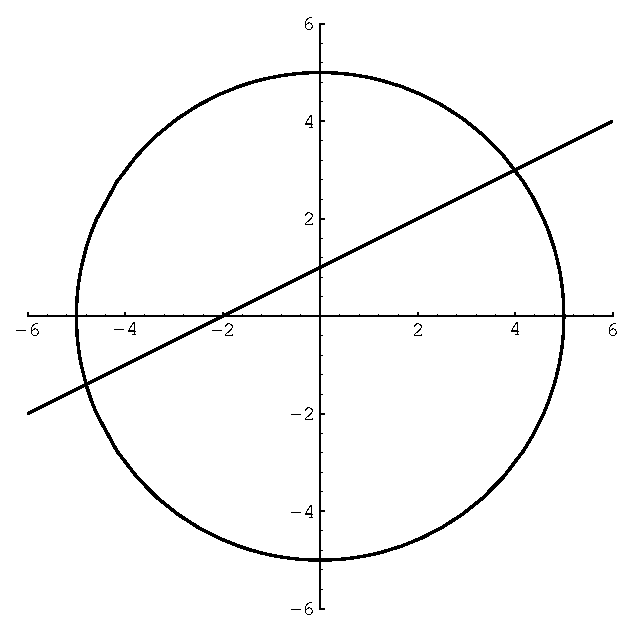
\includegraphics[width=3truein]{CircleLine}
\end{center}
\caption{Simple Algebraic Curves\label{Circle:Fig}}
\end{figure}

Let us start with the simplest type of geometric algebraic object, an
\keyi{algebraic curve}.  By an algebraic curve we mean a one-dimension
set of points whose coordinates satisfy an algebraic equation.  Two
simple examples of algebraic curves are shown in \figref{Circle:Fig},
where we have drawn a circle and straight line.  The points on the
circle are the zeroes of the polynomial $x^2 + y^2 - 25$, while the
line is the zeroes of $3y - x - 2$.  In particular we can define a
plane curve to be the set of zeroes of a polynomial in two variables.

Do the lines in \figref{Circle:Fig} constitute two curves or a single
curves?  It appears that it consists of two separate curves, one
superimposed on the other.  Nonetheless, there is a single polynomial
whose zeroes are the points in \figref{Circle:Fig}.  It is
\[
x^3 - 3 x^2 y + y^2 x - 3 y^3 + 2 x^2 + 2 y^2 - 25 x + 75 y + 50,
\]
which is the product of $x^2 + y^2 - 25$ and $3y - x - 2$.  We
probably want to say that the set of zeroes of an irreducible
polynomial is a single curve (or \keyi{irreducible curve}).

\begin{figure}
\begin{center}
  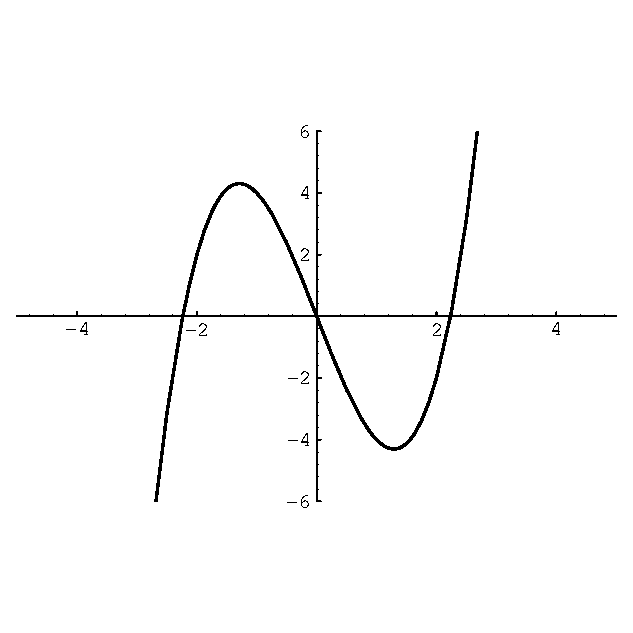
\includegraphics[width=1.5truein]{SimpleCubic1}
    \hfil 
  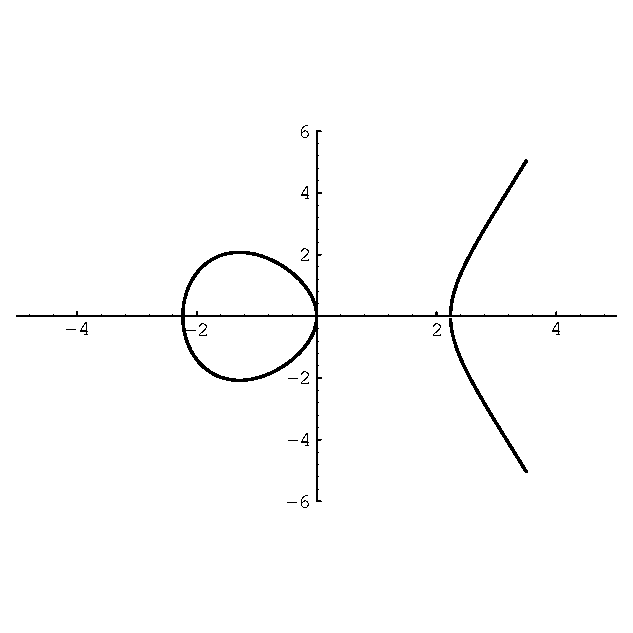
\includegraphics[width=1.5truein]{SimpleCubic2}
\end{center}
\caption{Cubic Curves: $y = x^3 - 5x$ and $y^2 = x^3 - 5x$}
\label{Simple:Cubic:Fig}
\end{figure}

Intuitively we think of the degree of an algebraic curve as the number of
times it can intersect a straight line.  For instance the curves in
\figref{Simple:Cubic:Fig} are obviously of degree three because each
intersects the $x$ axis at three places and no straight line can intersect
them more often.  Similarly the degree of the circle and straight line in
\figref{Circle:Fig} are 2 and 1 respectively.

Notice that a straight line can intersect a sine wave an infinite number of
times.  The sine wave is not an algebraic curve, if it was would have to be the
zeroes of a polynomial of infinite degree.  It is an example of a
transcendental curve.

The second curve of \figref{Simple:Cubic:Fig} is somewhat problematic.
It has two components, but the polynomial $y^2 - x^3 + 5x$ is
irreducible.  One way of looking at this curve is that it is generated
by taking the square roots of the values of $y$ in the
\figref{Simple:Cubic:Fig}(a).  Since there are two values of
$\sqrt{\alpha}$ for each value of $\alpha$, there are two values of
$y$ for each value of $x$ in \figref{Simple:Cubic:Fig}(b).  Notice
that the gap between the loop on the left and the curve on the right
at $x = \sqrt{5}$ arises because the the curve $x^3 - 5x$ is negative
in that region.  Thus the missing values actually lie in the complex
plane.

\begin{figure}
\begin{center}
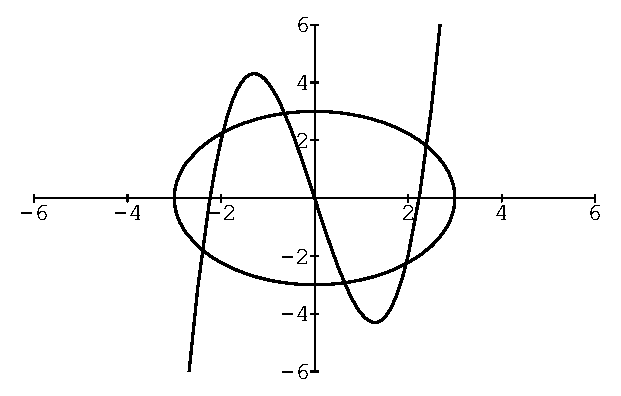
\includegraphics[width=3truein]{SimpIntersection}
\end{center}
\caption{Intersection of a Cubic and a Quadratic\label{Intersect:Fig}}
\end{figure}

Generalizing our observation on the intersection of curves and
straight lines, we would expect that the number of intersections of a
curve of degree $m$ and a curve of degree $n$ would be $mn$.  This is
illustrated by the curves in \figref{Intersect:Fig} where there are
six intersections.  Unfortunately is not always true.  Sometimes there
are fewer intersections.

\begin{figure}
\begin{center}
  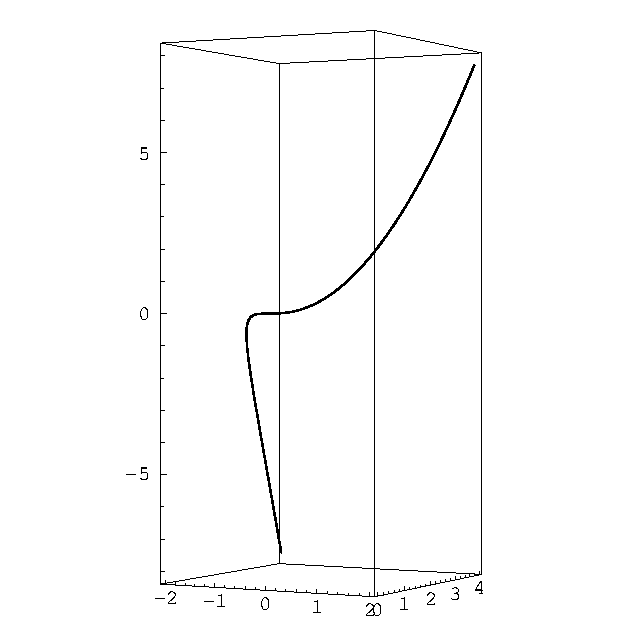
\includegraphics[width=1.5truein]{TwistedCubic1}
    \hfil 
  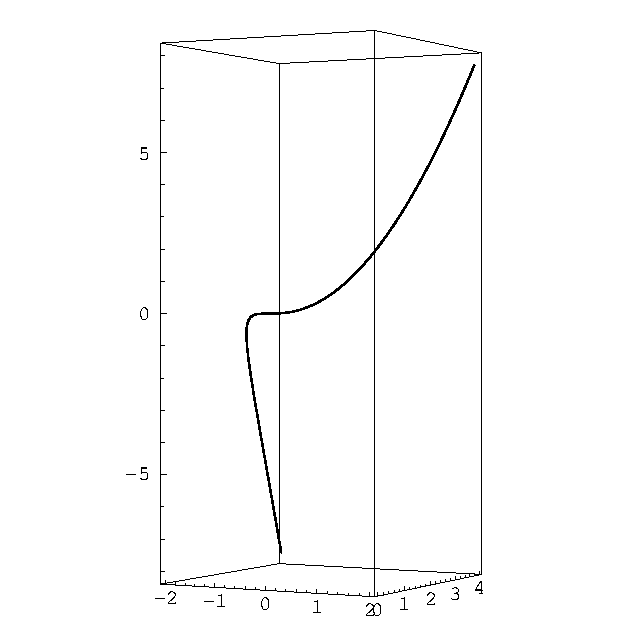
\includegraphics[width=1.5truein]{TwistedCubic2}
\end{center}
\caption{Twisted Cubic\label{Twisted:Cubic:Fig}}
\end{figure}
In three dimensions a single polynomial defines a surface.  In
general the intersection of two surfaces is a curve, although in
exceptional cases it could be a single point or a surface.  An example
of a curve in three dimensions is the \keyi{twisted cubic} shown in
\figref{Twisted:Cubic:Fig}.  This curve is the intersection of the surfaces
\[
y= x^2 \qquad \hbox{and}\qquad z=x^3.
\]
It is a fairly simple example of a curve that cannot be embedded in a
the plane.

\section{Commutative Algebra}

In the most general setting, we begin with a commutative ring $R$.  A
set of elements $I$ is chosen, and used to divide $R$ into equivalence
classes.  Two elements of $R$ are equivalent if their difference is in
$I$.  The set of equivalence classes is denoted by $R/I$.  We will
place restrictions on $I$ so that $R/I$ is still a ring.  For an
element to be equivalent to itself $0$ must be in $I$.  In fact, for
the relationship induced by $I$ to be an equivalence, $I$ must be an
additive group.  It is also not hard to see that if $i$ is an element
of $I$ and $a$ an element of $R$, then $ai$ must be an element of $I$.
Pick two elements of $R$, $r_1$ and $r_2$, such that $r_1 - r_2 = i$.
Since $r_1$ and $r_2$ are equivalent, we must have that $a r_1$ and
$ar_2$ are equivalent.  Thus, $$a r_1 - a r_2 = a \,(r_1 - r_2) = a i
\in I.$$ Sets that have these properties are called ideals.

\begin{definition}
Let $R$ be a commutative ring, and $I$ a subset of $R$.  If $I$ is an
additive group, and if $rI \subset I$ for all $r \in R$, then $I$ is
an \keyb{ideal}.
\end{definition}

\index{ideal, principal} \index{ideal, finitely generated}
In the integer case we used the set of multiples of an integer for
$I$.  The polynomial case described above used multiples of a single
polynomial $p(X)$.  Ideals that are multiples of a single element are
called {\em principal ideals\/}.  We have used the notation $(p)$ to
denote the set of multiples of $p$.  Generalizing this notation
slightly we will let $(a_1, a_2, \ldots, a_n)$ represent the set
\[
S = \{\, a_1 r_1 + a_2 r_2 + \cdots + a_n r_n 
        \mid r_1, r_2, \ldots, r_n \in R \,\}.
\]
$S$ is clearly an ideal. We say that $S$ is {\em generated} by $a_1,
a_2, \ldots, a_n$.  Since $S$ is generated by a finite number of
elements $S$ is called a {\em finitely generated ideal\/}.  There are
rings that have ideals which are not finitely generated, but we will
not discuss them here.  

All rings possess two ideals, the set consisting of the single element $0$
and the whole ring, $R$.  Notice that all the ideals of $R$ contain $(0)$
and are contained in $R$.  The residue class rings of these two ideals are
very dull ($R$ and zero ring) so most of our attention is confined to the
ideals between these two ``trivial'' ideals.

Recall that $\Z/(p)$ had no zero divisors if $p$ was a prime number.  In
fact $\Z/(p)$ is a field in this case.  We will extend
this definition to more general ideals.  Let $R$ be a ring, $I$ an ideal.
$I$ is a {\em prime ideal} if $R/I$ is an integral domain.  If $R/I$ is a
field then $I$ is a {\em maximal ideal\/}.  It is not difficult to see that
these characterizations are equivalent to standard definitions:

\begin{definition}
 $I$ is a \keyi{prime ideal} if for all elements $a$ and $b$
of $R$ such that $ab$ is an element of $I$, either $a$ or $b$ is an
element of $I$.
\end{definition}

\begin{definition}
$I$ is a \keyi{maximal ideal} if there is no ideal $J$ such that $I
\subset J$ other than $R$.
\end{definition}

All maximal ideals are prime.  For $\Z$ all prime ideals  are also maximal.
The situation is not always so simple.  If $R = \Z[X]$ there are three
classes of prime ideals: (p) where $p$ is a prime, $(f(X))$ where $f(X)$ is
an irreducible polynomial, and $(p, f(X))$ where $f(X)$ is irreducible
modulo $p$.  Only the third class leads to a field.

The set of prime ideals of a ring, $R$, is called the ring's
\keyi{spectrum}, $\Spec R$.  It is possible to put a topology on this
space called the \keyi{Zariski topology}.  The point of the space are then the
prime ideals.  Consider the ring $\Z[X]$.  Among the points in the
spectrum are the ideals generated by the linear polynomials $(X - a)$.
Thus there is a clear association between $\Z$ and a subset of the
points in $\Spec \Z$.  Similarly, there is an association between the
elements of $\Z \times \Z$ and the points of $\Spec \Z[X, Y]$.

Let $f$ be an element of $F[X]$, where $F$ is some field.  Let 
$\pger = (X - a)$ be a prime ideal of $F[X]$.  The residue of $f$ modulo
$\pger$ is $f(a)$.  In the spectrum of $F[X]$, the point $\pger$ is
associated with $a$ in $F$.  Thus it is natural to say that $f(a)$ is 
{\em the value of $f$ at $\pger$}.  More generally,
let $f$ be an element of some ring $R$ and $\pger$ a prime ideal of $R$.
The image of $f$ in $R/\pger$ is said to be the value of $f$ at $\pger$ and
is written $f(\pger)$ or $f_{\pger}$.

\medskip

\begin{definition}
A ring is said to be \keyi{Noetherian} if every ideal in the ring is
finitely generated.
\end{definition}

\begin{proposition}
Noetherian rings satisfy the descending chain condition.
\end{proposition}

\index{Hilbert Basis Theorem}
\begin{proposition}[Hilbert Basis Theorem] If $R$ is Noetherian then
$R[X]$ is also Noetherian.
\end{proposition}

\begin{proof}
Let $I$ be an ideal of $R[X]$.  The leading coefficients of the
elements of $I$ form an ideal in $R$ denoted by $\lc(I)$.  Since $R$
is noetherian $\lc(I)$ is finitely generated.  We will use this fact
to construct a basis for $I$.  Let $\{a_1, \ldots, a_n\}$ be a
generating set for $\lc(I)$.  Choose polynomials, $f_1, \ldots, f_n
\in I$ of smallest degree such that the leading coefficient of $f_i$
is $a_i$.  These polynomials generate an ideal $I' \subseteq I$.  Let
the maximum degree of any of the $f_i$ be $r$.  If $\deg f_i < r$,
replace $f$ by $X^{r -\deg f_i} f_i$ so that each of the $f_i$ is of
degree $r$.

We now show that the elements of $I$ are sums of elements of $I'$ and
polynomials of degree less than $r$.  Let $f = a X^m + \cdots$ be a
polynomial in $I$ but not $I'$, and assume $m \ge r$.  Since $\lc(I)$
is finitely generated, we can write $a$ as a linear combination of the
$a_i$
\[
a = c_1 a_1 + \cdots c_n a_n.
\]
The polynomial 
\[
g = X^{m-r} \left[ c_1 f_1 + \cdots c_n f_n \right]
\]
is an element of $I'$ and has the same leading term as $f$.  Repeating
this procedure with $f - g$ we can reduce $f$ to the sum of an element
in $I'$ and an element of $I$ of degree less than $r$.

Now we need to show that the elements of $I$ of degree less than $r$
are finitely generated.  Exactly the same technique is applied.  Let
$J_m$ denote the ideal of the leading coefficients of polynomials in
$I$ of degree $m$ and let $\{ f_{m1}, \ldots, f_{m n_m} \}$ be a set
of polynomials in $I$ of degree $m$ whose leading coefficients
generate $J_m$.  The finite set of polynomials $\{f_i \} \cap \{f_{ij}
\}$ generate $I$.

\end{proof}

The Hilbert Nullstellensatz.  Rabinowitsch's trick in \cite{Rabinowitsch29}.

\section{Ideal Theoretic Calculations}
\label{Ideal:Arith:Sec}

Given two orders $\ge_{x}$ and $\ge_{y}$ on monomials in $\vec X$ and
$\vec Y$ respectively, we can define an order on $\ge_{xy}$ by $\vec
X^{\vec a} \vec Y^{\vec b} \ge_{xy} \vec X^{\vec a'} \vec Y^{\vec b'}$
if $\vec X^{\vec a} \ge_{x} \vec X^{\vec a'}$ or $\vec X^{\vec a} =
\vec X^{\vec a'}$ and $\vec Y^{\vec b} \ge_{y} \vec Y^{\vec b'}$.

\begin{proposition}[Gianni-Trager-Zacharias]
\label{Lexical:Grobner:Prop}
Let $I$ be an ideal in $R[\vec X, \vec Y]$.  If $G \subset R[\vec X,
\vec Y]$ is a Gr\"obner basis for $I$ with respect to $\ge_{xy}$ then 
\begin{itemize}
\item $G$ is a Gr\"obner basis for $I$ with respect to the order
$\ge_x$ on $(R[\vec Y])[\vec X]$, the polynomial ring with coefficients
in $R[\vec Y]$.
\item $G\cap R[\vec Y]$ is a Gr\"obner basis for $I\cap R[y]$ with
respect to the order $\ge_{y}$.
\end{itemize}
\end{proposition}


\subsection{Ideal Arithmetic}
\label{Ideal:Arithmetic:Sec}

Compute intersection, quotient, dimension, localization of an ideal.

\subsection{Primary Decomposition}

\begin{proposition}[Gianni-Trager-Zacharias]
Let $I$ be a prime zero-dimensional ideal in $k[\vec X]$, 
\[
G = \{g_1(X_1, \ldots, X_n), g_2(X_2, \ldots, X_n), \ldots, g_n(X_n)\}
\]
a minimal Gr\"obner basis for $I$ with respect to $\lexord$.  Then for
almost all linear transformations of coordinates $g_i$ is linear in
$X_i$ for all $i$ less than $n$.
\end{proposition}

\begin{proof}
By the proof of the primitive element theorem, for almost all $a_1,
\ldots, a_n \in k$,
\[
R = k[\vec X]/I \simeq k[a_1 X_1 + \cdots + a_n X_n].
\]
If we choose new coordinates $Z_1, \ldots, Z_n$ such that 
\[
Z_n = a_1 X_1 + \cdots + a_n X_n
\]
then $R = k[Z_n]$.  Since $Z_i \in R$, $Z_i = f_i(Z_n)$ for some
polynomial $f_i$.
\end{proof}

\section{Special Case Lifting Techniques}



